% Created by tikzDevice version 0.7.0 on 2014-07-29 02:50:04
% !TEX encoding = UTF-8 Unicode
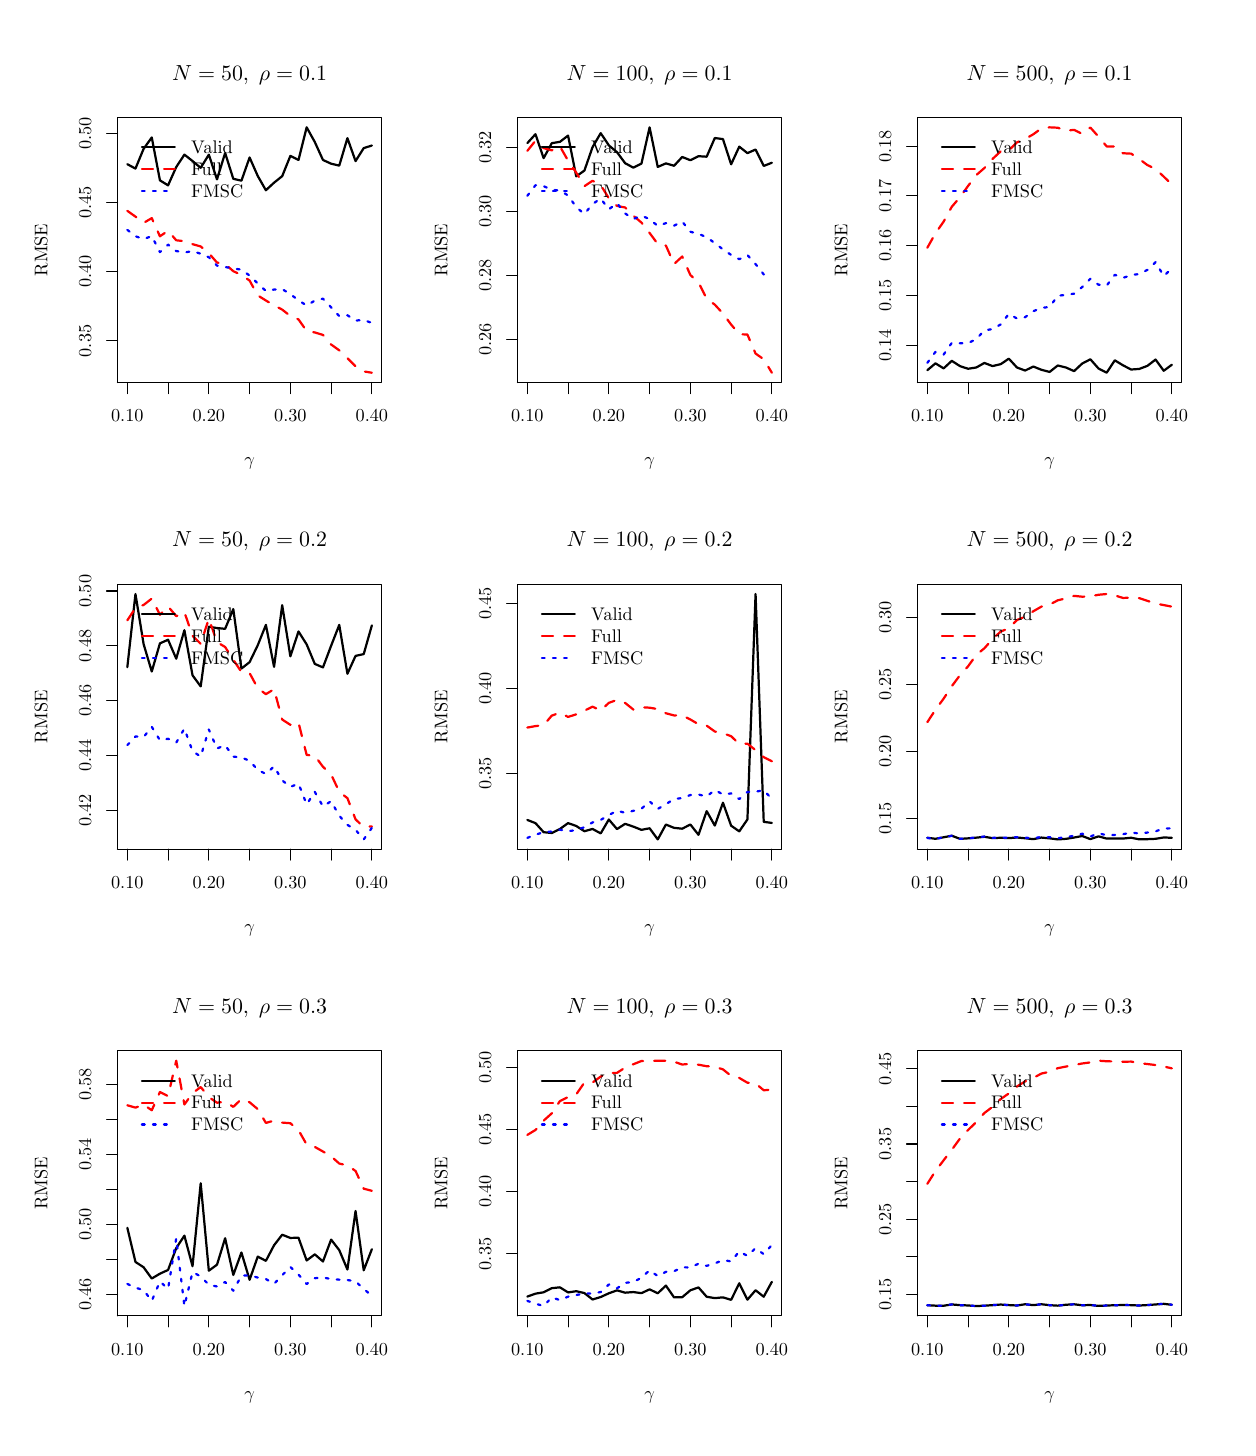
\begin{tikzpicture}[x=1pt,y=1pt]
\definecolor[named]{fillColor}{rgb}{1.00,1.00,1.00}
\path[use as bounding box,fill=fillColor,fill opacity=0.00] (0,0) rectangle (433.62,505.89);
\begin{scope}
\path[clip] ( 32.47,377.65) rectangle (127.91,473.42);
\definecolor[named]{drawColor}{rgb}{0.00,0.00,0.00}

\path[draw=drawColor,line width= 0.8pt,line join=round,line cap=round] ( 36.01,456.55) --
	( 38.95,454.97) --
	( 41.90,462.13) --
	( 44.84,466.21) --
	( 47.79,450.72) --
	( 50.73,448.91) --
	( 53.68,455.52) --
	( 56.63,460.01) --
	( 59.57,457.70) --
	( 62.52,455.24) --
	( 65.46,460.00) --
	( 68.41,451.06) --
	( 71.35,460.60) --
	( 74.30,451.27) --
	( 77.24,450.59) --
	( 80.19,458.98) --
	( 83.14,452.29) --
	( 86.08,447.14) --
	( 89.03,449.87) --
	( 91.97,452.23) --
	( 94.92,459.55) --
	( 97.86,458.07) --
	(100.81,469.87) --
	(103.75,464.57) --
	(106.70,458.08) --
	(109.65,456.73) --
	(112.59,456.04) --
	(115.54,465.97) --
	(118.48,457.68) --
	(121.43,462.37) --
	(124.37,463.30);
\end{scope}
\begin{scope}
\path[clip] (  0.00,  0.00) rectangle (433.62,505.89);
\definecolor[named]{drawColor}{rgb}{0.00,0.00,0.00}

\path[draw=drawColor,line width= 0.4pt,line join=round,line cap=round] ( 36.01,377.65) -- (124.37,377.65);

\path[draw=drawColor,line width= 0.4pt,line join=round,line cap=round] ( 36.01,377.65) -- ( 36.01,373.69);

\path[draw=drawColor,line width= 0.4pt,line join=round,line cap=round] ( 50.73,377.65) -- ( 50.73,373.69);

\path[draw=drawColor,line width= 0.4pt,line join=round,line cap=round] ( 65.46,377.65) -- ( 65.46,373.69);

\path[draw=drawColor,line width= 0.4pt,line join=round,line cap=round] ( 80.19,377.65) -- ( 80.19,373.69);

\path[draw=drawColor,line width= 0.4pt,line join=round,line cap=round] ( 94.92,377.65) -- ( 94.92,373.69);

\path[draw=drawColor,line width= 0.4pt,line join=round,line cap=round] (109.65,377.65) -- (109.65,373.69);

\path[draw=drawColor,line width= 0.4pt,line join=round,line cap=round] (124.37,377.65) -- (124.37,373.69);

\node[text=drawColor,anchor=base,inner sep=0pt, outer sep=0pt, scale=  0.66] at ( 36.01,363.40) {0.10};

\node[text=drawColor,anchor=base,inner sep=0pt, outer sep=0pt, scale=  0.66] at ( 65.46,363.40) {0.20};

\node[text=drawColor,anchor=base,inner sep=0pt, outer sep=0pt, scale=  0.66] at ( 94.92,363.40) {0.30};

\node[text=drawColor,anchor=base,inner sep=0pt, outer sep=0pt, scale=  0.66] at (124.37,363.40) {0.40};

\path[draw=drawColor,line width= 0.4pt,line join=round,line cap=round] ( 32.47,392.70) -- ( 32.47,467.73);

\path[draw=drawColor,line width= 0.4pt,line join=round,line cap=round] ( 32.47,392.70) -- ( 28.51,392.70);

\path[draw=drawColor,line width= 0.4pt,line join=round,line cap=round] ( 32.47,417.71) -- ( 28.51,417.71);

\path[draw=drawColor,line width= 0.4pt,line join=round,line cap=round] ( 32.47,442.72) -- ( 28.51,442.72);

\path[draw=drawColor,line width= 0.4pt,line join=round,line cap=round] ( 32.47,467.73) -- ( 28.51,467.73);

\node[text=drawColor,rotate= 90.00,anchor=base,inner sep=0pt, outer sep=0pt, scale=  0.66] at ( 22.97,392.70) {0.35};

\node[text=drawColor,rotate= 90.00,anchor=base,inner sep=0pt, outer sep=0pt, scale=  0.66] at ( 22.97,417.71) {0.40};

\node[text=drawColor,rotate= 90.00,anchor=base,inner sep=0pt, outer sep=0pt, scale=  0.66] at ( 22.97,442.72) {0.45};

\node[text=drawColor,rotate= 90.00,anchor=base,inner sep=0pt, outer sep=0pt, scale=  0.66] at ( 22.97,467.73) {0.50};

\path[draw=drawColor,line width= 0.4pt,line join=round,line cap=round] ( 32.47,377.65) --
	(127.91,377.65) --
	(127.91,473.42) --
	( 32.47,473.42) --
	( 32.47,377.65);
\end{scope}
\begin{scope}
\path[clip] (  0.00,337.26) rectangle (144.54,505.89);
\definecolor[named]{drawColor}{rgb}{0.00,0.00,0.00}

\node[text=drawColor,anchor=base,inner sep=0pt, outer sep=0pt, scale=  0.79] at ( 80.19,486.92) {\bfseries $N=50, \;\rho=0.1$};

\node[text=drawColor,anchor=base,inner sep=0pt, outer sep=0pt, scale=  0.66] at ( 80.19,347.56) {$\gamma$};

\node[text=drawColor,rotate= 90.00,anchor=base,inner sep=0pt, outer sep=0pt, scale=  0.66] at (  7.13,425.53) {RMSE};
\end{scope}
\begin{scope}
\path[clip] ( 32.47,377.65) rectangle (127.91,473.42);
\definecolor[named]{drawColor}{rgb}{1.00,0.00,0.00}

\path[draw=drawColor,line width= 0.8pt,dash pattern=on 4pt off 4pt ,line join=round,line cap=round] ( 36.01,439.70) --
	( 38.95,437.61) --
	( 41.90,435.35) --
	( 44.84,437.06) --
	( 47.79,430.50) --
	( 50.73,432.48) --
	( 53.68,429.06) --
	( 56.63,428.72) --
	( 59.57,427.66) --
	( 62.52,426.83) --
	( 65.46,424.39) --
	( 68.41,421.01) --
	( 71.35,420.48) --
	( 74.30,417.89) --
	( 77.24,416.53) --
	( 80.19,414.50) --
	( 83.14,409.14) --
	( 86.08,407.29) --
	( 89.03,405.54) --
	( 91.97,404.01) --
	( 94.92,401.68) --
	( 97.86,400.47) --
	(100.81,396.27) --
	(103.75,395.76) --
	(106.70,394.86) --
	(109.65,391.40) --
	(112.59,389.29) --
	(115.54,386.45) --
	(118.48,383.52) --
	(121.43,381.68) --
	(124.37,381.20);
\definecolor[named]{drawColor}{rgb}{0.00,0.00,1.00}

\path[draw=drawColor,line width= 0.8pt,dash pattern=on 1pt off 3pt ,line join=round,line cap=round] ( 36.01,432.81) --
	( 38.95,430.50) --
	( 41.90,429.50) --
	( 44.84,430.56) --
	( 47.79,424.78) --
	( 50.73,427.50) --
	( 53.68,425.16) --
	( 56.63,424.66) --
	( 59.57,425.12) --
	( 62.52,424.20) --
	( 65.46,422.93) --
	( 68.41,419.91) --
	( 71.35,419.40) --
	( 74.30,418.86) --
	( 77.24,418.45) --
	( 80.19,416.30) --
	( 83.14,413.47) --
	( 86.08,410.73) --
	( 89.03,411.25) --
	( 91.97,411.41) --
	( 94.92,409.60) --
	( 97.86,407.37) --
	(100.81,405.48) --
	(103.75,407.26) --
	(106.70,407.95) --
	(109.65,404.82) --
	(112.59,401.65) --
	(115.54,401.96) --
	(118.48,400.05) --
	(121.43,400.27) --
	(124.37,399.18);
\definecolor[named]{drawColor}{rgb}{0.00,0.00,0.00}

\path[draw=drawColor,line width= 0.8pt,line join=round,line cap=round] ( 41.28,462.63) -- ( 53.16,462.63);
\definecolor[named]{drawColor}{rgb}{1.00,0.00,0.00}

\path[draw=drawColor,line width= 0.8pt,dash pattern=on 4pt off 4pt ,line join=round,line cap=round] ( 41.28,454.71) -- ( 53.16,454.71);
\definecolor[named]{drawColor}{rgb}{0.00,0.00,1.00}

\path[draw=drawColor,line width= 0.8pt,dash pattern=on 1pt off 3pt ,line join=round,line cap=round] ( 41.28,446.79) -- ( 53.16,446.79);
\definecolor[named]{drawColor}{rgb}{0.00,0.00,0.00}

\node[text=drawColor,anchor=base west,inner sep=0pt, outer sep=0pt, scale=  0.66] at ( 59.10,460.35) {Valid};

\node[text=drawColor,anchor=base west,inner sep=0pt, outer sep=0pt, scale=  0.66] at ( 59.10,452.43) {Full};

\node[text=drawColor,anchor=base west,inner sep=0pt, outer sep=0pt, scale=  0.66] at ( 59.10,444.51) {FMSC};
\end{scope}
\begin{scope}
\path[clip] (177.01,377.65) rectangle (272.45,473.42);
\definecolor[named]{drawColor}{rgb}{0.00,0.00,0.00}

\path[draw=drawColor,line width= 0.8pt,line join=round,line cap=round] (180.55,464.17) --
	(183.49,467.39) --
	(186.44,458.74) --
	(189.38,464.14) --
	(192.33,464.63) --
	(195.27,466.89) --
	(198.22,452.17) --
	(201.17,454.24) --
	(204.11,462.71) --
	(207.06,467.76) --
	(210.00,463.36) --
	(212.95,460.90) --
	(215.89,456.91) --
	(218.84,455.31) --
	(221.78,456.75) --
	(224.73,469.87) --
	(227.68,455.56) --
	(230.62,456.85) --
	(233.57,455.98) --
	(236.51,459.16) --
	(239.46,457.99) --
	(242.40,459.44) --
	(245.35,459.26) --
	(248.29,466.01) --
	(251.24,465.62) --
	(254.19,456.51) --
	(257.13,462.89) --
	(260.08,460.55) --
	(263.02,461.85) --
	(265.97,455.92) --
	(268.91,457.08);
\end{scope}
\begin{scope}
\path[clip] (  0.00,  0.00) rectangle (433.62,505.89);
\definecolor[named]{drawColor}{rgb}{0.00,0.00,0.00}

\path[draw=drawColor,line width= 0.4pt,line join=round,line cap=round] (180.55,377.65) -- (268.91,377.65);

\path[draw=drawColor,line width= 0.4pt,line join=round,line cap=round] (180.55,377.65) -- (180.55,373.69);

\path[draw=drawColor,line width= 0.4pt,line join=round,line cap=round] (195.27,377.65) -- (195.27,373.69);

\path[draw=drawColor,line width= 0.4pt,line join=round,line cap=round] (210.00,377.65) -- (210.00,373.69);

\path[draw=drawColor,line width= 0.4pt,line join=round,line cap=round] (224.73,377.65) -- (224.73,373.69);

\path[draw=drawColor,line width= 0.4pt,line join=round,line cap=round] (239.46,377.65) -- (239.46,373.69);

\path[draw=drawColor,line width= 0.4pt,line join=round,line cap=round] (254.19,377.65) -- (254.19,373.69);

\path[draw=drawColor,line width= 0.4pt,line join=round,line cap=round] (268.91,377.65) -- (268.91,373.69);

\node[text=drawColor,anchor=base,inner sep=0pt, outer sep=0pt, scale=  0.66] at (180.55,363.40) {0.10};

\node[text=drawColor,anchor=base,inner sep=0pt, outer sep=0pt, scale=  0.66] at (210.00,363.40) {0.20};

\node[text=drawColor,anchor=base,inner sep=0pt, outer sep=0pt, scale=  0.66] at (239.46,363.40) {0.30};

\node[text=drawColor,anchor=base,inner sep=0pt, outer sep=0pt, scale=  0.66] at (268.91,363.40) {0.40};

\path[draw=drawColor,line width= 0.4pt,line join=round,line cap=round] (177.01,393.34) -- (177.01,462.58);

\path[draw=drawColor,line width= 0.4pt,line join=round,line cap=round] (177.01,393.34) -- (173.05,393.34);

\path[draw=drawColor,line width= 0.4pt,line join=round,line cap=round] (177.01,416.42) -- (173.05,416.42);

\path[draw=drawColor,line width= 0.4pt,line join=round,line cap=round] (177.01,439.50) -- (173.05,439.50);

\path[draw=drawColor,line width= 0.4pt,line join=round,line cap=round] (177.01,462.58) -- (173.05,462.58);

\node[text=drawColor,rotate= 90.00,anchor=base,inner sep=0pt, outer sep=0pt, scale=  0.66] at (167.51,393.34) {0.26};

\node[text=drawColor,rotate= 90.00,anchor=base,inner sep=0pt, outer sep=0pt, scale=  0.66] at (167.51,416.42) {0.28};

\node[text=drawColor,rotate= 90.00,anchor=base,inner sep=0pt, outer sep=0pt, scale=  0.66] at (167.51,439.50) {0.30};

\node[text=drawColor,rotate= 90.00,anchor=base,inner sep=0pt, outer sep=0pt, scale=  0.66] at (167.51,462.58) {0.32};

\path[draw=drawColor,line width= 0.4pt,line join=round,line cap=round] (177.01,377.65) --
	(272.45,377.65) --
	(272.45,473.42) --
	(177.01,473.42) --
	(177.01,377.65);
\end{scope}
\begin{scope}
\path[clip] (144.54,337.26) rectangle (289.08,505.89);
\definecolor[named]{drawColor}{rgb}{0.00,0.00,0.00}

\node[text=drawColor,anchor=base,inner sep=0pt, outer sep=0pt, scale=  0.79] at (224.73,486.92) {\bfseries $N=100, \;\rho=0.1$};

\node[text=drawColor,anchor=base,inner sep=0pt, outer sep=0pt, scale=  0.66] at (224.73,347.56) {$\gamma$};

\node[text=drawColor,rotate= 90.00,anchor=base,inner sep=0pt, outer sep=0pt, scale=  0.66] at (151.67,425.53) {RMSE};
\end{scope}
\begin{scope}
\path[clip] (177.01,377.65) rectangle (272.45,473.42);
\definecolor[named]{drawColor}{rgb}{1.00,0.00,0.00}

\path[draw=drawColor,line width= 0.8pt,dash pattern=on 4pt off 4pt ,line join=round,line cap=round] (180.55,461.37) --
	(183.49,465.02) --
	(186.44,462.37) --
	(189.38,461.55) --
	(192.33,462.99) --
	(195.27,457.83) --
	(198.22,453.50) --
	(201.17,448.59) --
	(204.11,450.55) --
	(207.06,449.02) --
	(210.00,444.25) --
	(212.95,441.47) --
	(215.89,440.91) --
	(218.84,437.92) --
	(221.78,435.47) --
	(224.73,431.70) --
	(227.68,427.72) --
	(230.62,427.14) --
	(233.57,420.48) --
	(236.51,423.19) --
	(239.46,416.51) --
	(242.40,413.85) --
	(245.35,407.95) --
	(248.29,405.80) --
	(251.24,402.59) --
	(254.19,398.60) --
	(257.13,395.14) --
	(260.08,394.98) --
	(263.02,388.13) --
	(265.97,386.05) --
	(268.91,381.20);
\definecolor[named]{drawColor}{rgb}{0.00,0.00,1.00}

\path[draw=drawColor,line width= 0.8pt,dash pattern=on 1pt off 3pt ,line join=round,line cap=round] (180.55,445.14) --
	(183.49,448.94) --
	(186.44,448.61) --
	(189.38,447.27) --
	(192.33,447.08) --
	(195.27,445.25) --
	(198.22,441.03) --
	(201.17,438.54) --
	(204.11,442.15) --
	(207.06,444.14) --
	(210.00,440.25) --
	(212.95,442.46) --
	(215.89,438.75) --
	(218.84,436.73) --
	(221.78,437.98) --
	(224.73,436.69) --
	(227.68,434.22) --
	(230.62,435.26) --
	(233.57,434.34) --
	(236.51,435.82) --
	(239.46,432.14) --
	(242.40,431.38) --
	(245.35,430.17) --
	(248.29,428.04) --
	(251.24,425.76) --
	(254.19,423.77) --
	(257.13,422.22) --
	(260.08,423.72) --
	(263.02,420.45) --
	(265.97,416.73) --
	(268.91,415.83);
\definecolor[named]{drawColor}{rgb}{0.00,0.00,0.00}

\path[draw=drawColor,line width= 0.8pt,line join=round,line cap=round] (185.82,462.63) -- (197.70,462.63);
\definecolor[named]{drawColor}{rgb}{1.00,0.00,0.00}

\path[draw=drawColor,line width= 0.8pt,dash pattern=on 4pt off 4pt ,line join=round,line cap=round] (185.82,454.71) -- (197.70,454.71);
\definecolor[named]{drawColor}{rgb}{0.00,0.00,1.00}

\path[draw=drawColor,line width= 0.8pt,dash pattern=on 1pt off 3pt ,line join=round,line cap=round] (185.82,446.79) -- (197.70,446.79);
\definecolor[named]{drawColor}{rgb}{0.00,0.00,0.00}

\node[text=drawColor,anchor=base west,inner sep=0pt, outer sep=0pt, scale=  0.66] at (203.64,460.35) {Valid};

\node[text=drawColor,anchor=base west,inner sep=0pt, outer sep=0pt, scale=  0.66] at (203.64,452.43) {Full};

\node[text=drawColor,anchor=base west,inner sep=0pt, outer sep=0pt, scale=  0.66] at (203.64,444.51) {FMSC};
\end{scope}
\begin{scope}
\path[clip] (321.55,377.65) rectangle (416.99,473.42);
\definecolor[named]{drawColor}{rgb}{0.00,0.00,0.00}

\path[draw=drawColor,line width= 0.8pt,line join=round,line cap=round] (325.09,382.11) --
	(328.03,384.59) --
	(330.98,382.77) --
	(333.92,385.50) --
	(336.87,383.60) --
	(339.81,382.63) --
	(342.76,383.09) --
	(345.71,384.73) --
	(348.65,383.60) --
	(351.60,384.30) --
	(354.54,386.28) --
	(357.49,383.08) --
	(360.43,381.99) --
	(363.38,383.44) --
	(366.32,382.26) --
	(369.27,381.48) --
	(372.22,383.82) --
	(375.16,383.09) --
	(378.11,381.78) --
	(381.05,384.52) --
	(384.00,386.06) --
	(386.94,382.73) --
	(389.89,381.20) --
	(392.83,385.69) --
	(395.78,383.88) --
	(398.73,382.36) --
	(401.67,382.57) --
	(404.62,383.69) --
	(407.56,385.96) --
	(410.51,381.91) --
	(413.45,384.09);
\end{scope}
\begin{scope}
\path[clip] (  0.00,  0.00) rectangle (433.62,505.89);
\definecolor[named]{drawColor}{rgb}{0.00,0.00,0.00}

\path[draw=drawColor,line width= 0.4pt,line join=round,line cap=round] (325.09,377.65) -- (413.45,377.65);

\path[draw=drawColor,line width= 0.4pt,line join=round,line cap=round] (325.09,377.65) -- (325.09,373.69);

\path[draw=drawColor,line width= 0.4pt,line join=round,line cap=round] (339.81,377.65) -- (339.81,373.69);

\path[draw=drawColor,line width= 0.4pt,line join=round,line cap=round] (354.54,377.65) -- (354.54,373.69);

\path[draw=drawColor,line width= 0.4pt,line join=round,line cap=round] (369.27,377.65) -- (369.27,373.69);

\path[draw=drawColor,line width= 0.4pt,line join=round,line cap=round] (384.00,377.65) -- (384.00,373.69);

\path[draw=drawColor,line width= 0.4pt,line join=round,line cap=round] (398.73,377.65) -- (398.73,373.69);

\path[draw=drawColor,line width= 0.4pt,line join=round,line cap=round] (413.45,377.65) -- (413.45,373.69);

\node[text=drawColor,anchor=base,inner sep=0pt, outer sep=0pt, scale=  0.66] at (325.09,363.40) {0.10};

\node[text=drawColor,anchor=base,inner sep=0pt, outer sep=0pt, scale=  0.66] at (354.54,363.40) {0.20};

\node[text=drawColor,anchor=base,inner sep=0pt, outer sep=0pt, scale=  0.66] at (384.00,363.40) {0.30};

\node[text=drawColor,anchor=base,inner sep=0pt, outer sep=0pt, scale=  0.66] at (413.45,363.40) {0.40};

\path[draw=drawColor,line width= 0.4pt,line join=round,line cap=round] (321.55,391.17) -- (321.55,463.05);

\path[draw=drawColor,line width= 0.4pt,line join=round,line cap=round] (321.55,391.17) -- (317.59,391.17);

\path[draw=drawColor,line width= 0.4pt,line join=round,line cap=round] (321.55,409.14) -- (317.59,409.14);

\path[draw=drawColor,line width= 0.4pt,line join=round,line cap=round] (321.55,427.11) -- (317.59,427.11);

\path[draw=drawColor,line width= 0.4pt,line join=round,line cap=round] (321.55,445.08) -- (317.59,445.08);

\path[draw=drawColor,line width= 0.4pt,line join=round,line cap=round] (321.55,463.05) -- (317.59,463.05);

\node[text=drawColor,rotate= 90.00,anchor=base,inner sep=0pt, outer sep=0pt, scale=  0.66] at (312.05,391.17) {0.14};

\node[text=drawColor,rotate= 90.00,anchor=base,inner sep=0pt, outer sep=0pt, scale=  0.66] at (312.05,409.14) {0.15};

\node[text=drawColor,rotate= 90.00,anchor=base,inner sep=0pt, outer sep=0pt, scale=  0.66] at (312.05,427.11) {0.16};

\node[text=drawColor,rotate= 90.00,anchor=base,inner sep=0pt, outer sep=0pt, scale=  0.66] at (312.05,445.08) {0.17};

\node[text=drawColor,rotate= 90.00,anchor=base,inner sep=0pt, outer sep=0pt, scale=  0.66] at (312.05,463.05) {0.18};

\path[draw=drawColor,line width= 0.4pt,line join=round,line cap=round] (321.55,377.65) --
	(416.99,377.65) --
	(416.99,473.42) --
	(321.55,473.42) --
	(321.55,377.65);
\end{scope}
\begin{scope}
\path[clip] (289.08,337.26) rectangle (433.62,505.89);
\definecolor[named]{drawColor}{rgb}{0.00,0.00,0.00}

\node[text=drawColor,anchor=base,inner sep=0pt, outer sep=0pt, scale=  0.79] at (369.27,486.92) {\bfseries $N=500, \;\rho=0.1$};

\node[text=drawColor,anchor=base,inner sep=0pt, outer sep=0pt, scale=  0.66] at (369.27,347.56) {$\gamma$};

\node[text=drawColor,rotate= 90.00,anchor=base,inner sep=0pt, outer sep=0pt, scale=  0.66] at (296.21,425.54) {RMSE};
\end{scope}
\begin{scope}
\path[clip] (321.55,377.65) rectangle (416.99,473.42);
\definecolor[named]{drawColor}{rgb}{1.00,0.00,0.00}

\path[draw=drawColor,line width= 0.8pt,dash pattern=on 4pt off 4pt ,line join=round,line cap=round] (325.09,426.36) --
	(328.03,431.60) --
	(330.98,435.81) --
	(333.92,441.16) --
	(336.87,444.61) --
	(339.81,448.70) --
	(342.76,452.59) --
	(345.71,455.17) --
	(348.65,458.45) --
	(351.60,461.20) --
	(354.54,461.55) --
	(357.49,464.45) --
	(360.43,465.66) --
	(363.38,467.36) --
	(366.32,469.51) --
	(369.27,469.87) --
	(372.22,469.73) --
	(375.16,468.66) --
	(378.11,468.96) --
	(381.05,467.50) --
	(384.00,469.79) --
	(386.94,466.49) --
	(389.89,462.98) --
	(392.83,462.97) --
	(395.78,460.51) --
	(398.73,460.36) --
	(401.67,458.43) --
	(404.62,456.23) --
	(407.56,454.80) --
	(410.51,452.07) --
	(413.45,449.20);
\definecolor[named]{drawColor}{rgb}{0.00,0.00,1.00}

\path[draw=drawColor,line width= 0.8pt,dash pattern=on 1pt off 3pt ,line join=round,line cap=round] (325.09,384.78) --
	(328.03,388.72) --
	(330.98,387.78) --
	(333.92,391.98) --
	(336.87,391.87) --
	(339.81,391.89) --
	(342.76,393.34) --
	(345.71,396.50) --
	(348.65,396.98) --
	(351.60,398.65) --
	(354.54,402.46) --
	(357.49,400.78) --
	(360.43,401.27) --
	(363.38,403.43) --
	(366.32,404.62) --
	(369.27,404.97) --
	(372.22,409.01) --
	(375.16,409.33) --
	(378.11,409.78) --
	(381.05,412.16) --
	(384.00,415.15) --
	(386.94,413.01) --
	(389.89,412.68) --
	(392.83,416.58) --
	(395.78,415.46) --
	(398.73,416.47) --
	(401.67,416.88) --
	(404.62,418.37) --
	(407.56,421.13) --
	(410.51,416.14) --
	(413.45,418.89);
\definecolor[named]{drawColor}{rgb}{0.00,0.00,0.00}

\path[draw=drawColor,line width= 0.8pt,line join=round,line cap=round] (330.36,462.63) -- (342.24,462.63);
\definecolor[named]{drawColor}{rgb}{1.00,0.00,0.00}

\path[draw=drawColor,line width= 0.8pt,dash pattern=on 4pt off 4pt ,line join=round,line cap=round] (330.36,454.71) -- (342.24,454.71);
\definecolor[named]{drawColor}{rgb}{0.00,0.00,1.00}

\path[draw=drawColor,line width= 0.8pt,dash pattern=on 1pt off 3pt ,line join=round,line cap=round] (330.36,446.79) -- (342.24,446.79);
\definecolor[named]{drawColor}{rgb}{0.00,0.00,0.00}

\node[text=drawColor,anchor=base west,inner sep=0pt, outer sep=0pt, scale=  0.66] at (348.18,460.35) {Valid};

\node[text=drawColor,anchor=base west,inner sep=0pt, outer sep=0pt, scale=  0.66] at (348.18,452.43) {Full};

\node[text=drawColor,anchor=base west,inner sep=0pt, outer sep=0pt, scale=  0.66] at (348.18,444.51) {FMSC};
\end{scope}
\begin{scope}
\path[clip] ( 32.47,209.02) rectangle (127.91,304.79);
\definecolor[named]{drawColor}{rgb}{0.00,0.00,0.00}

\path[draw=drawColor,line width= 0.8pt,line join=round,line cap=round] ( 36.01,274.80) --
	( 38.95,301.24) --
	( 41.90,283.11) --
	( 44.84,273.23) --
	( 47.79,283.41) --
	( 50.73,284.71) --
	( 53.68,277.87) --
	( 56.63,288.17) --
	( 59.57,271.86) --
	( 62.52,267.85) --
	( 65.46,289.41) --
	( 68.41,288.94) --
	( 71.35,288.66) --
	( 74.30,295.80) --
	( 77.24,274.30) --
	( 80.19,276.62) --
	( 83.14,282.73) --
	( 86.08,290.09) --
	( 89.03,274.92) --
	( 91.97,297.20) --
	( 94.92,278.71) --
	( 97.86,287.71) --
	(100.81,283.03) --
	(103.75,275.98) --
	(106.70,274.72) --
	(109.65,282.55) --
	(112.59,290.08) --
	(115.54,272.42) --
	(118.48,278.88) --
	(121.43,279.53) --
	(124.37,289.90);
\end{scope}
\begin{scope}
\path[clip] (  0.00,  0.00) rectangle (433.62,505.89);
\definecolor[named]{drawColor}{rgb}{0.00,0.00,0.00}

\path[draw=drawColor,line width= 0.4pt,line join=round,line cap=round] ( 36.01,209.02) -- (124.37,209.02);

\path[draw=drawColor,line width= 0.4pt,line join=round,line cap=round] ( 36.01,209.02) -- ( 36.01,205.06);

\path[draw=drawColor,line width= 0.4pt,line join=round,line cap=round] ( 50.73,209.02) -- ( 50.73,205.06);

\path[draw=drawColor,line width= 0.4pt,line join=round,line cap=round] ( 65.46,209.02) -- ( 65.46,205.06);

\path[draw=drawColor,line width= 0.4pt,line join=round,line cap=round] ( 80.19,209.02) -- ( 80.19,205.06);

\path[draw=drawColor,line width= 0.4pt,line join=round,line cap=round] ( 94.92,209.02) -- ( 94.92,205.06);

\path[draw=drawColor,line width= 0.4pt,line join=round,line cap=round] (109.65,209.02) -- (109.65,205.06);

\path[draw=drawColor,line width= 0.4pt,line join=round,line cap=round] (124.37,209.02) -- (124.37,205.06);

\node[text=drawColor,anchor=base,inner sep=0pt, outer sep=0pt, scale=  0.66] at ( 36.01,194.77) {0.10};

\node[text=drawColor,anchor=base,inner sep=0pt, outer sep=0pt, scale=  0.66] at ( 65.46,194.77) {0.20};

\node[text=drawColor,anchor=base,inner sep=0pt, outer sep=0pt, scale=  0.66] at ( 94.92,194.77) {0.30};

\node[text=drawColor,anchor=base,inner sep=0pt, outer sep=0pt, scale=  0.66] at (124.37,194.77) {0.40};

\path[draw=drawColor,line width= 0.4pt,line join=round,line cap=round] ( 32.47,223.06) -- ( 32.47,302.31);

\path[draw=drawColor,line width= 0.4pt,line join=round,line cap=round] ( 32.47,223.06) -- ( 28.51,223.06);

\path[draw=drawColor,line width= 0.4pt,line join=round,line cap=round] ( 32.47,242.87) -- ( 28.51,242.87);

\path[draw=drawColor,line width= 0.4pt,line join=round,line cap=round] ( 32.47,262.68) -- ( 28.51,262.68);

\path[draw=drawColor,line width= 0.4pt,line join=round,line cap=round] ( 32.47,282.49) -- ( 28.51,282.49);

\path[draw=drawColor,line width= 0.4pt,line join=round,line cap=round] ( 32.47,302.31) -- ( 28.51,302.31);

\node[text=drawColor,rotate= 90.00,anchor=base,inner sep=0pt, outer sep=0pt, scale=  0.66] at ( 22.97,223.06) {0.42};

\node[text=drawColor,rotate= 90.00,anchor=base,inner sep=0pt, outer sep=0pt, scale=  0.66] at ( 22.97,242.87) {0.44};

\node[text=drawColor,rotate= 90.00,anchor=base,inner sep=0pt, outer sep=0pt, scale=  0.66] at ( 22.97,262.68) {0.46};

\node[text=drawColor,rotate= 90.00,anchor=base,inner sep=0pt, outer sep=0pt, scale=  0.66] at ( 22.97,282.49) {0.48};

\node[text=drawColor,rotate= 90.00,anchor=base,inner sep=0pt, outer sep=0pt, scale=  0.66] at ( 22.97,302.31) {0.50};

\path[draw=drawColor,line width= 0.4pt,line join=round,line cap=round] ( 32.47,209.02) --
	(127.91,209.02) --
	(127.91,304.79) --
	( 32.47,304.79) --
	( 32.47,209.02);
\end{scope}
\begin{scope}
\path[clip] (  0.00,168.63) rectangle (144.54,337.26);
\definecolor[named]{drawColor}{rgb}{0.00,0.00,0.00}

\node[text=drawColor,anchor=base,inner sep=0pt, outer sep=0pt, scale=  0.79] at ( 80.19,318.29) {\bfseries $N=50, \;\rho=0.2$};

\node[text=drawColor,anchor=base,inner sep=0pt, outer sep=0pt, scale=  0.66] at ( 80.19,178.93) {$\gamma$};

\node[text=drawColor,rotate= 90.00,anchor=base,inner sep=0pt, outer sep=0pt, scale=  0.66] at (  7.13,256.90) {RMSE};
\end{scope}
\begin{scope}
\path[clip] ( 32.47,209.02) rectangle (127.91,304.79);
\definecolor[named]{drawColor}{rgb}{1.00,0.00,0.00}

\path[draw=drawColor,line width= 0.8pt,dash pattern=on 4pt off 4pt ,line join=round,line cap=round] ( 36.01,291.74) --
	( 38.95,296.19) --
	( 41.90,297.28) --
	( 44.84,299.59) --
	( 47.79,293.74) --
	( 50.73,296.75) --
	( 53.68,293.24) --
	( 56.63,294.70) --
	( 59.57,286.14) --
	( 62.52,283.26) --
	( 65.46,292.34) --
	( 68.41,283.86) --
	( 71.35,282.09) --
	( 74.30,277.49) --
	( 77.24,273.05) --
	( 80.19,272.65) --
	( 83.14,267.22) --
	( 86.08,265.05) --
	( 89.03,266.85) --
	( 91.97,255.88) --
	( 94.92,253.98) --
	( 97.86,254.79) --
	(100.81,243.10) --
	(103.75,242.79) --
	(106.70,238.82) --
	(109.65,236.04) --
	(112.59,229.78) --
	(115.54,227.47) --
	(118.48,219.80) --
	(121.43,217.04) --
	(124.37,217.28);
\definecolor[named]{drawColor}{rgb}{0.00,0.00,1.00}

\path[draw=drawColor,line width= 0.8pt,dash pattern=on 1pt off 3pt ,line join=round,line cap=round] ( 36.01,246.65) --
	( 38.95,249.76) --
	( 41.90,249.55) --
	( 44.84,253.24) --
	( 47.79,248.40) --
	( 50.73,248.93) --
	( 53.68,247.52) --
	( 56.63,252.61) --
	( 59.57,244.46) --
	( 62.52,242.50) --
	( 65.46,252.27) --
	( 68.41,245.42) --
	( 71.35,246.60) --
	( 74.30,242.48) --
	( 77.24,242.18) --
	( 80.19,240.97) --
	( 83.14,237.68) --
	( 86.08,236.22) --
	( 89.03,238.96) --
	( 91.97,233.89) --
	( 94.92,231.53) --
	( 97.86,232.73) --
	(100.81,225.22) --
	(103.75,229.73) --
	(106.70,224.50) --
	(109.65,226.38) --
	(112.59,221.10) --
	(115.54,217.82) --
	(118.48,216.02) --
	(121.43,212.57) --
	(124.37,216.74);
\definecolor[named]{drawColor}{rgb}{0.00,0.00,0.00}

\path[draw=drawColor,line width= 0.8pt,line join=round,line cap=round] ( 41.28,294.00) -- ( 53.16,294.00);
\definecolor[named]{drawColor}{rgb}{1.00,0.00,0.00}

\path[draw=drawColor,line width= 0.8pt,dash pattern=on 4pt off 4pt ,line join=round,line cap=round] ( 41.28,286.08) -- ( 53.16,286.08);
\definecolor[named]{drawColor}{rgb}{0.00,0.00,1.00}

\path[draw=drawColor,line width= 0.8pt,dash pattern=on 1pt off 3pt ,line join=round,line cap=round] ( 41.28,278.16) -- ( 53.16,278.16);
\definecolor[named]{drawColor}{rgb}{0.00,0.00,0.00}

\node[text=drawColor,anchor=base west,inner sep=0pt, outer sep=0pt, scale=  0.66] at ( 59.10,291.72) {Valid};

\node[text=drawColor,anchor=base west,inner sep=0pt, outer sep=0pt, scale=  0.66] at ( 59.10,283.80) {Full};

\node[text=drawColor,anchor=base west,inner sep=0pt, outer sep=0pt, scale=  0.66] at ( 59.10,275.88) {FMSC};
\end{scope}
\begin{scope}
\path[clip] (177.01,209.02) rectangle (272.45,304.79);
\definecolor[named]{drawColor}{rgb}{0.00,0.00,0.00}

\path[draw=drawColor,line width= 0.8pt,line join=round,line cap=round] (180.55,219.60) --
	(183.49,218.45) --
	(186.44,215.18) --
	(189.38,214.88) --
	(192.33,216.33) --
	(195.27,218.46) --
	(198.22,217.42) --
	(201.17,215.52) --
	(204.11,216.34) --
	(207.06,214.74) --
	(210.00,219.75) --
	(212.95,216.30) --
	(215.89,218.20) --
	(218.84,217.19) --
	(221.78,216.02) --
	(224.73,216.59) --
	(227.68,212.57) --
	(230.62,217.94) --
	(233.57,216.74) --
	(236.51,216.44) --
	(239.46,217.95) --
	(242.40,214.23) --
	(245.35,222.79) --
	(248.29,217.56) --
	(251.24,225.83) --
	(254.19,217.52) --
	(257.13,215.48) --
	(260.08,219.78) --
	(263.02,301.24) --
	(265.97,218.92) --
	(268.91,218.52);
\end{scope}
\begin{scope}
\path[clip] (  0.00,  0.00) rectangle (433.62,505.89);
\definecolor[named]{drawColor}{rgb}{0.00,0.00,0.00}

\path[draw=drawColor,line width= 0.4pt,line join=round,line cap=round] (180.55,209.02) -- (268.91,209.02);

\path[draw=drawColor,line width= 0.4pt,line join=round,line cap=round] (180.55,209.02) -- (180.55,205.06);

\path[draw=drawColor,line width= 0.4pt,line join=round,line cap=round] (195.27,209.02) -- (195.27,205.06);

\path[draw=drawColor,line width= 0.4pt,line join=round,line cap=round] (210.00,209.02) -- (210.00,205.06);

\path[draw=drawColor,line width= 0.4pt,line join=round,line cap=round] (224.73,209.02) -- (224.73,205.06);

\path[draw=drawColor,line width= 0.4pt,line join=round,line cap=round] (239.46,209.02) -- (239.46,205.06);

\path[draw=drawColor,line width= 0.4pt,line join=round,line cap=round] (254.19,209.02) -- (254.19,205.06);

\path[draw=drawColor,line width= 0.4pt,line join=round,line cap=round] (268.91,209.02) -- (268.91,205.06);

\node[text=drawColor,anchor=base,inner sep=0pt, outer sep=0pt, scale=  0.66] at (180.55,194.77) {0.10};

\node[text=drawColor,anchor=base,inner sep=0pt, outer sep=0pt, scale=  0.66] at (210.00,194.77) {0.20};

\node[text=drawColor,anchor=base,inner sep=0pt, outer sep=0pt, scale=  0.66] at (239.46,194.77) {0.30};

\node[text=drawColor,anchor=base,inner sep=0pt, outer sep=0pt, scale=  0.66] at (268.91,194.77) {0.40};

\path[draw=drawColor,line width= 0.4pt,line join=round,line cap=round] (177.01,236.38) -- (177.01,297.75);

\path[draw=drawColor,line width= 0.4pt,line join=round,line cap=round] (177.01,236.38) -- (173.05,236.38);

\path[draw=drawColor,line width= 0.4pt,line join=round,line cap=round] (177.01,267.07) -- (173.05,267.07);

\path[draw=drawColor,line width= 0.4pt,line join=round,line cap=round] (177.01,297.75) -- (173.05,297.75);

\node[text=drawColor,rotate= 90.00,anchor=base,inner sep=0pt, outer sep=0pt, scale=  0.66] at (167.51,236.38) {0.35};

\node[text=drawColor,rotate= 90.00,anchor=base,inner sep=0pt, outer sep=0pt, scale=  0.66] at (167.51,267.07) {0.40};

\node[text=drawColor,rotate= 90.00,anchor=base,inner sep=0pt, outer sep=0pt, scale=  0.66] at (167.51,297.75) {0.45};

\path[draw=drawColor,line width= 0.4pt,line join=round,line cap=round] (177.01,209.02) --
	(272.45,209.02) --
	(272.45,304.79) --
	(177.01,304.79) --
	(177.01,209.02);
\end{scope}
\begin{scope}
\path[clip] (144.54,168.63) rectangle (289.08,337.26);
\definecolor[named]{drawColor}{rgb}{0.00,0.00,0.00}

\node[text=drawColor,anchor=base,inner sep=0pt, outer sep=0pt, scale=  0.79] at (224.73,318.29) {\bfseries $N=100, \;\rho=0.2$};

\node[text=drawColor,anchor=base,inner sep=0pt, outer sep=0pt, scale=  0.66] at (224.73,178.93) {$\gamma$};

\node[text=drawColor,rotate= 90.00,anchor=base,inner sep=0pt, outer sep=0pt, scale=  0.66] at (151.67,256.90) {RMSE};
\end{scope}
\begin{scope}
\path[clip] (177.01,209.02) rectangle (272.45,304.79);
\definecolor[named]{drawColor}{rgb}{1.00,0.00,0.00}

\path[draw=drawColor,line width= 0.8pt,dash pattern=on 4pt off 4pt ,line join=round,line cap=round] (180.55,252.98) --
	(183.49,253.51) --
	(186.44,253.84) --
	(189.38,257.28) --
	(192.33,258.37) --
	(195.27,256.82) --
	(198.22,257.77) --
	(201.17,259.09) --
	(204.11,260.53) --
	(207.06,259.14) --
	(210.00,261.91) --
	(212.95,262.98) --
	(215.89,261.88) --
	(218.84,259.50) --
	(221.78,260.33) --
	(224.73,260.16) --
	(227.68,259.65) --
	(230.62,258.15) --
	(233.57,257.37) --
	(236.51,257.42) --
	(239.46,255.89) --
	(242.40,254.18) --
	(245.35,253.68) --
	(248.29,251.56) --
	(251.24,250.96) --
	(254.19,249.86) --
	(257.13,247.05) --
	(260.08,247.18) --
	(263.02,244.81) --
	(265.97,242.30) --
	(268.91,240.79);
\definecolor[named]{drawColor}{rgb}{0.00,0.00,1.00}

\path[draw=drawColor,line width= 0.8pt,dash pattern=on 1pt off 3pt ,line join=round,line cap=round] (180.55,213.12) --
	(183.49,214.23) --
	(186.44,215.23) --
	(189.38,215.42) --
	(192.33,216.08) --
	(195.27,215.54) --
	(198.22,215.92) --
	(201.17,216.98) --
	(204.11,218.69) --
	(207.06,219.61) --
	(210.00,221.34) --
	(212.95,222.97) --
	(215.89,222.16) --
	(218.84,222.90) --
	(221.78,223.64) --
	(224.73,226.34) --
	(227.68,223.58) --
	(230.62,225.31) --
	(233.57,227.15) --
	(236.51,227.51) --
	(239.46,228.60) --
	(242.40,228.79) --
	(245.35,228.07) --
	(248.29,230.43) --
	(251.24,228.80) --
	(254.19,229.19) --
	(257.13,227.14) --
	(260.08,229.71) --
	(263.02,229.80) --
	(265.97,230.34) --
	(268.91,227.19);
\definecolor[named]{drawColor}{rgb}{0.00,0.00,0.00}

\path[draw=drawColor,line width= 0.8pt,line join=round,line cap=round] (185.82,294.00) -- (197.70,294.00);
\definecolor[named]{drawColor}{rgb}{1.00,0.00,0.00}

\path[draw=drawColor,line width= 0.8pt,dash pattern=on 4pt off 4pt ,line join=round,line cap=round] (185.82,286.08) -- (197.70,286.08);
\definecolor[named]{drawColor}{rgb}{0.00,0.00,1.00}

\path[draw=drawColor,line width= 0.8pt,dash pattern=on 1pt off 3pt ,line join=round,line cap=round] (185.82,278.16) -- (197.70,278.16);
\definecolor[named]{drawColor}{rgb}{0.00,0.00,0.00}

\node[text=drawColor,anchor=base west,inner sep=0pt, outer sep=0pt, scale=  0.66] at (203.64,291.72) {Valid};

\node[text=drawColor,anchor=base west,inner sep=0pt, outer sep=0pt, scale=  0.66] at (203.64,283.80) {Full};

\node[text=drawColor,anchor=base west,inner sep=0pt, outer sep=0pt, scale=  0.66] at (203.64,275.88) {FMSC};
\end{scope}
\begin{scope}
\path[clip] (321.55,209.02) rectangle (416.99,304.79);
\definecolor[named]{drawColor}{rgb}{0.00,0.00,0.00}

\path[draw=drawColor,line width= 0.8pt,line join=round,line cap=round] (325.09,213.16) --
	(328.03,212.79) --
	(330.98,213.34) --
	(333.92,213.90) --
	(336.87,212.77) --
	(339.81,212.95) --
	(342.76,213.20) --
	(345.71,213.51) --
	(348.65,213.03) --
	(351.60,213.16) --
	(354.54,213.04) --
	(357.49,213.25) --
	(360.43,212.98) --
	(363.38,212.66) --
	(366.32,213.23) --
	(369.27,212.95) --
	(372.22,212.57) --
	(375.16,212.77) --
	(378.11,213.24) --
	(381.05,213.79) --
	(384.00,212.67) --
	(386.94,213.68) --
	(389.89,212.86) --
	(392.83,212.87) --
	(395.78,212.88) --
	(398.73,213.17) --
	(401.67,212.59) --
	(404.62,212.65) --
	(407.56,212.78) --
	(410.51,213.27) --
	(413.45,213.15);
\end{scope}
\begin{scope}
\path[clip] (  0.00,  0.00) rectangle (433.62,505.89);
\definecolor[named]{drawColor}{rgb}{0.00,0.00,0.00}

\path[draw=drawColor,line width= 0.4pt,line join=round,line cap=round] (325.09,209.02) -- (413.45,209.02);

\path[draw=drawColor,line width= 0.4pt,line join=round,line cap=round] (325.09,209.02) -- (325.09,205.06);

\path[draw=drawColor,line width= 0.4pt,line join=round,line cap=round] (339.81,209.02) -- (339.81,205.06);

\path[draw=drawColor,line width= 0.4pt,line join=round,line cap=round] (354.54,209.02) -- (354.54,205.06);

\path[draw=drawColor,line width= 0.4pt,line join=round,line cap=round] (369.27,209.02) -- (369.27,205.06);

\path[draw=drawColor,line width= 0.4pt,line join=round,line cap=round] (384.00,209.02) -- (384.00,205.06);

\path[draw=drawColor,line width= 0.4pt,line join=round,line cap=round] (398.73,209.02) -- (398.73,205.06);

\path[draw=drawColor,line width= 0.4pt,line join=round,line cap=round] (413.45,209.02) -- (413.45,205.06);

\node[text=drawColor,anchor=base,inner sep=0pt, outer sep=0pt, scale=  0.66] at (325.09,194.77) {0.10};

\node[text=drawColor,anchor=base,inner sep=0pt, outer sep=0pt, scale=  0.66] at (354.54,194.77) {0.20};

\node[text=drawColor,anchor=base,inner sep=0pt, outer sep=0pt, scale=  0.66] at (384.00,194.77) {0.30};

\node[text=drawColor,anchor=base,inner sep=0pt, outer sep=0pt, scale=  0.66] at (413.45,194.77) {0.40};

\path[draw=drawColor,line width= 0.4pt,line join=round,line cap=round] (321.55,220.08) -- (321.55,292.71);

\path[draw=drawColor,line width= 0.4pt,line join=round,line cap=round] (321.55,220.08) -- (317.59,220.08);

\path[draw=drawColor,line width= 0.4pt,line join=round,line cap=round] (321.55,244.29) -- (317.59,244.29);

\path[draw=drawColor,line width= 0.4pt,line join=round,line cap=round] (321.55,268.50) -- (317.59,268.50);

\path[draw=drawColor,line width= 0.4pt,line join=round,line cap=round] (321.55,292.71) -- (317.59,292.71);

\node[text=drawColor,rotate= 90.00,anchor=base,inner sep=0pt, outer sep=0pt, scale=  0.66] at (312.05,220.08) {0.15};

\node[text=drawColor,rotate= 90.00,anchor=base,inner sep=0pt, outer sep=0pt, scale=  0.66] at (312.05,244.29) {0.20};

\node[text=drawColor,rotate= 90.00,anchor=base,inner sep=0pt, outer sep=0pt, scale=  0.66] at (312.05,268.50) {0.25};

\node[text=drawColor,rotate= 90.00,anchor=base,inner sep=0pt, outer sep=0pt, scale=  0.66] at (312.05,292.71) {0.30};

\path[draw=drawColor,line width= 0.4pt,line join=round,line cap=round] (321.55,209.02) --
	(416.99,209.02) --
	(416.99,304.79) --
	(321.55,304.79) --
	(321.55,209.02);
\end{scope}
\begin{scope}
\path[clip] (289.08,168.63) rectangle (433.62,337.26);
\definecolor[named]{drawColor}{rgb}{0.00,0.00,0.00}

\node[text=drawColor,anchor=base,inner sep=0pt, outer sep=0pt, scale=  0.79] at (369.27,318.29) {\bfseries $N=500, \;\rho=0.2$};

\node[text=drawColor,anchor=base,inner sep=0pt, outer sep=0pt, scale=  0.66] at (369.27,178.93) {$\gamma$};

\node[text=drawColor,rotate= 90.00,anchor=base,inner sep=0pt, outer sep=0pt, scale=  0.66] at (296.21,256.90) {RMSE};
\end{scope}
\begin{scope}
\path[clip] (321.55,209.02) rectangle (416.99,304.79);
\definecolor[named]{drawColor}{rgb}{1.00,0.00,0.00}

\path[draw=drawColor,line width= 0.8pt,dash pattern=on 4pt off 4pt ,line join=round,line cap=round] (325.09,254.93) --
	(328.03,259.43) --
	(330.98,263.44) --
	(333.92,267.92) --
	(336.87,271.87) --
	(339.81,275.11) --
	(342.76,279.22) --
	(345.71,281.63) --
	(348.65,284.97) --
	(351.60,287.67) --
	(354.54,288.86) --
	(357.49,291.86) --
	(360.43,293.05) --
	(363.38,295.01) --
	(366.32,296.69) --
	(369.27,297.41) --
	(372.22,298.96) --
	(375.16,299.67) --
	(378.11,300.57) --
	(381.05,300.27) --
	(384.00,300.40) --
	(386.94,300.97) --
	(389.89,301.24) --
	(392.83,300.74) --
	(395.78,299.82) --
	(398.73,299.92) --
	(401.67,299.75) --
	(404.62,298.76) --
	(407.56,297.81) --
	(410.51,297.24) --
	(413.45,296.67);
\definecolor[named]{drawColor}{rgb}{0.00,0.00,1.00}

\path[draw=drawColor,line width= 0.8pt,dash pattern=on 1pt off 3pt ,line join=round,line cap=round] (325.09,213.10) --
	(328.03,212.74) --
	(330.98,213.34) --
	(333.92,213.87) --
	(336.87,212.78) --
	(339.81,212.99) --
	(342.76,213.25) --
	(345.71,213.61) --
	(348.65,213.11) --
	(351.60,213.24) --
	(354.54,213.16) --
	(357.49,213.37) --
	(360.43,213.21) --
	(363.38,212.94) --
	(366.32,213.50) --
	(369.27,213.35) --
	(372.22,213.01) --
	(375.16,213.37) --
	(378.11,213.89) --
	(381.05,214.62) --
	(384.00,213.62) --
	(386.94,214.79) --
	(389.89,214.06) --
	(392.83,214.20) --
	(395.78,214.45) --
	(398.73,215.03) --
	(401.67,214.72) --
	(404.62,215.04) --
	(407.56,215.48) --
	(410.51,216.53) --
	(413.45,216.56);
\definecolor[named]{drawColor}{rgb}{0.00,0.00,0.00}

\path[draw=drawColor,line width= 0.8pt,line join=round,line cap=round] (330.36,294.00) -- (342.24,294.00);
\definecolor[named]{drawColor}{rgb}{1.00,0.00,0.00}

\path[draw=drawColor,line width= 0.8pt,dash pattern=on 4pt off 4pt ,line join=round,line cap=round] (330.36,286.08) -- (342.24,286.08);
\definecolor[named]{drawColor}{rgb}{0.00,0.00,1.00}

\path[draw=drawColor,line width= 0.8pt,dash pattern=on 1pt off 3pt ,line join=round,line cap=round] (330.36,278.16) -- (342.24,278.16);
\definecolor[named]{drawColor}{rgb}{0.00,0.00,0.00}

\node[text=drawColor,anchor=base west,inner sep=0pt, outer sep=0pt, scale=  0.66] at (348.18,291.72) {Valid};

\node[text=drawColor,anchor=base west,inner sep=0pt, outer sep=0pt, scale=  0.66] at (348.18,283.80) {Full};

\node[text=drawColor,anchor=base west,inner sep=0pt, outer sep=0pt, scale=  0.66] at (348.18,275.88) {FMSC};
\end{scope}
\begin{scope}
\path[clip] ( 32.47, 40.39) rectangle (127.91,136.16);
\definecolor[named]{drawColor}{rgb}{0.00,0.00,0.00}

\path[draw=drawColor,line width= 0.8pt,line join=round,line cap=round] ( 36.01, 72.22) --
	( 38.95, 59.90) --
	( 41.90, 57.94) --
	( 44.84, 53.89) --
	( 47.79, 55.65) --
	( 50.73, 56.98) --
	( 53.68, 64.89) --
	( 56.63, 69.39) --
	( 59.57, 58.33) --
	( 62.52, 88.31) --
	( 65.46, 56.72) --
	( 68.41, 58.89) --
	( 71.35, 68.45) --
	( 74.30, 55.18) --
	( 77.24, 63.31) --
	( 80.19, 53.43) --
	( 83.14, 61.82) --
	( 86.08, 60.28) --
	( 89.03, 65.92) --
	( 91.97, 69.72) --
	( 94.92, 68.56) --
	( 97.86, 68.64) --
	(100.81, 60.41) --
	(103.75, 62.63) --
	(106.70, 60.05) --
	(109.65, 67.96) --
	(112.59, 64.15) --
	(115.54, 57.14) --
	(118.48, 78.30) --
	(121.43, 56.88) --
	(124.37, 64.49);
\end{scope}
\begin{scope}
\path[clip] (  0.00,  0.00) rectangle (433.62,505.89);
\definecolor[named]{drawColor}{rgb}{0.00,0.00,0.00}

\path[draw=drawColor,line width= 0.4pt,line join=round,line cap=round] ( 36.01, 40.39) -- (124.37, 40.39);

\path[draw=drawColor,line width= 0.4pt,line join=round,line cap=round] ( 36.01, 40.39) -- ( 36.01, 36.43);

\path[draw=drawColor,line width= 0.4pt,line join=round,line cap=round] ( 50.73, 40.39) -- ( 50.73, 36.43);

\path[draw=drawColor,line width= 0.4pt,line join=round,line cap=round] ( 65.46, 40.39) -- ( 65.46, 36.43);

\path[draw=drawColor,line width= 0.4pt,line join=round,line cap=round] ( 80.19, 40.39) -- ( 80.19, 36.43);

\path[draw=drawColor,line width= 0.4pt,line join=round,line cap=round] ( 94.92, 40.39) -- ( 94.92, 36.43);

\path[draw=drawColor,line width= 0.4pt,line join=round,line cap=round] (109.65, 40.39) -- (109.65, 36.43);

\path[draw=drawColor,line width= 0.4pt,line join=round,line cap=round] (124.37, 40.39) -- (124.37, 36.43);

\node[text=drawColor,anchor=base,inner sep=0pt, outer sep=0pt, scale=  0.66] at ( 36.01, 26.14) {0.10};

\node[text=drawColor,anchor=base,inner sep=0pt, outer sep=0pt, scale=  0.66] at ( 65.46, 26.14) {0.20};

\node[text=drawColor,anchor=base,inner sep=0pt, outer sep=0pt, scale=  0.66] at ( 94.92, 26.14) {0.30};

\node[text=drawColor,anchor=base,inner sep=0pt, outer sep=0pt, scale=  0.66] at (124.37, 26.14) {0.40};

\path[draw=drawColor,line width= 0.4pt,line join=round,line cap=round] ( 32.47, 48.23) -- ( 32.47,123.97);

\path[draw=drawColor,line width= 0.4pt,line join=round,line cap=round] ( 32.47, 48.23) -- ( 28.51, 48.23);

\path[draw=drawColor,line width= 0.4pt,line join=round,line cap=round] ( 32.47, 60.85) -- ( 28.51, 60.85);

\path[draw=drawColor,line width= 0.4pt,line join=round,line cap=round] ( 32.47, 73.48) -- ( 28.51, 73.48);

\path[draw=drawColor,line width= 0.4pt,line join=round,line cap=round] ( 32.47, 86.10) -- ( 28.51, 86.10);

\path[draw=drawColor,line width= 0.4pt,line join=round,line cap=round] ( 32.47, 98.72) -- ( 28.51, 98.72);

\path[draw=drawColor,line width= 0.4pt,line join=round,line cap=round] ( 32.47,111.35) -- ( 28.51,111.35);

\path[draw=drawColor,line width= 0.4pt,line join=round,line cap=round] ( 32.47,123.97) -- ( 28.51,123.97);

\node[text=drawColor,rotate= 90.00,anchor=base,inner sep=0pt, outer sep=0pt, scale=  0.66] at ( 22.97, 48.23) {0.46};

\node[text=drawColor,rotate= 90.00,anchor=base,inner sep=0pt, outer sep=0pt, scale=  0.66] at ( 22.97, 73.48) {0.50};

\node[text=drawColor,rotate= 90.00,anchor=base,inner sep=0pt, outer sep=0pt, scale=  0.66] at ( 22.97, 98.72) {0.54};

\node[text=drawColor,rotate= 90.00,anchor=base,inner sep=0pt, outer sep=0pt, scale=  0.66] at ( 22.97,123.97) {0.58};

\path[draw=drawColor,line width= 0.4pt,line join=round,line cap=round] ( 32.47, 40.39) --
	(127.91, 40.39) --
	(127.91,136.16) --
	( 32.47,136.16) --
	( 32.47, 40.39);
\end{scope}
\begin{scope}
\path[clip] (  0.00,  0.00) rectangle (144.54,168.63);
\definecolor[named]{drawColor}{rgb}{0.00,0.00,0.00}

\node[text=drawColor,anchor=base,inner sep=0pt, outer sep=0pt, scale=  0.79] at ( 80.19,149.66) {\bfseries $N=50, \;\rho=0.3$};

\node[text=drawColor,anchor=base,inner sep=0pt, outer sep=0pt, scale=  0.66] at ( 80.19, 10.30) {$\gamma$};

\node[text=drawColor,rotate= 90.00,anchor=base,inner sep=0pt, outer sep=0pt, scale=  0.66] at (  7.13, 88.28) {RMSE};
\end{scope}
\begin{scope}
\path[clip] ( 32.47, 40.39) rectangle (127.91,136.16);
\definecolor[named]{drawColor}{rgb}{1.00,0.00,0.00}

\path[draw=drawColor,line width= 0.8pt,dash pattern=on 4pt off 4pt ,line join=round,line cap=round] ( 36.01,116.50) --
	( 38.95,115.65) --
	( 41.90,116.75) --
	( 44.84,114.69) --
	( 47.79,121.29) --
	( 50.73,119.79) --
	( 53.68,132.61) --
	( 56.63,116.79) --
	( 59.57,120.85) --
	( 62.52,123.09) --
	( 65.46,119.46) --
	( 68.41,117.41) --
	( 71.35,117.82) --
	( 74.30,115.92) --
	( 77.24,118.76) --
	( 80.19,117.59) --
	( 83.14,115.09) --
	( 86.08,110.12) --
	( 89.03,110.97) --
	( 91.97,110.24) --
	( 94.92,110.01) --
	( 97.86,107.52) --
	(100.81,102.31) --
	(103.75,101.45) --
	(106.70, 99.79) --
	(109.65, 98.04) --
	(112.59, 95.44) --
	(115.54, 94.74) --
	(118.48, 92.76) --
	(121.43, 86.36) --
	(124.37, 85.59);
\definecolor[named]{drawColor}{rgb}{0.00,0.00,1.00}

\path[draw=drawColor,line width= 0.8pt,dash pattern=on 1pt off 3pt ,line join=round,line cap=round] ( 36.01, 51.94) --
	( 38.95, 50.60) --
	( 41.90, 49.69) --
	( 44.84, 45.81) --
	( 47.79, 52.84) --
	( 50.73, 50.16) --
	( 53.68, 68.42) --
	( 56.63, 43.94) --
	( 59.57, 56.19) --
	( 62.52, 54.67) --
	( 65.46, 51.62) --
	( 68.41, 51.02) --
	( 71.35, 52.63) --
	( 74.30, 49.49) --
	( 77.24, 54.95) --
	( 80.19, 55.04) --
	( 83.14, 54.24) --
	( 86.08, 53.71) --
	( 89.03, 51.96) --
	( 91.97, 55.08) --
	( 94.92, 58.06) --
	( 97.86, 55.32) --
	(100.81, 51.91) --
	(103.75, 54.01) --
	(106.70, 54.26) --
	(109.65, 53.72) --
	(112.59, 53.48) --
	(115.54, 53.35) --
	(118.48, 52.88) --
	(121.43, 50.08) --
	(124.37, 47.73);
\definecolor[named]{drawColor}{rgb}{0.00,0.00,0.00}

\path[draw=drawColor,line width= 0.8pt,line join=round,line cap=round] ( 41.28,125.37) -- ( 53.16,125.37);
\definecolor[named]{drawColor}{rgb}{1.00,0.00,0.00}

\path[draw=drawColor,line width= 0.8pt,dash pattern=on 4pt off 4pt ,line join=round,line cap=round] ( 41.28,117.45) -- ( 53.16,117.45);
\definecolor[named]{drawColor}{rgb}{0.00,0.00,1.00}

\path[draw=drawColor,line width= 0.8pt,dash pattern=on 1pt off 3pt ,line join=round,line cap=round] ( 41.28,109.53) -- ( 53.16,109.53);
\definecolor[named]{drawColor}{rgb}{0.00,0.00,0.00}

\node[text=drawColor,anchor=base west,inner sep=0pt, outer sep=0pt, scale=  0.66] at ( 59.10,123.09) {Valid};

\node[text=drawColor,anchor=base west,inner sep=0pt, outer sep=0pt, scale=  0.66] at ( 59.10,115.17) {Full};

\node[text=drawColor,anchor=base west,inner sep=0pt, outer sep=0pt, scale=  0.66] at ( 59.10,107.25) {FMSC};
\end{scope}
\begin{scope}
\path[clip] (177.01, 40.39) rectangle (272.45,136.16);
\definecolor[named]{drawColor}{rgb}{0.00,0.00,0.00}

\path[draw=drawColor,line width= 0.8pt,line join=round,line cap=round] (180.55, 47.37) --
	(183.49, 48.42) --
	(186.44, 48.92) --
	(189.38, 50.41) --
	(192.33, 50.71) --
	(195.27, 48.87) --
	(198.22, 49.31) --
	(201.17, 48.64) --
	(204.11, 46.32) --
	(207.06, 47.21) --
	(210.00, 48.56) --
	(212.95, 49.62) --
	(215.89, 48.78) --
	(218.84, 49.00) --
	(221.78, 48.61) --
	(224.73, 49.98) --
	(227.68, 48.56) --
	(230.62, 51.34) --
	(233.57, 47.08) --
	(236.51, 47.14) --
	(239.46, 49.64) --
	(242.40, 50.68) --
	(245.35, 47.31) --
	(248.29, 46.81) --
	(251.24, 47.09) --
	(254.19, 46.19) --
	(257.13, 52.17) --
	(260.08, 46.25) --
	(263.02, 49.66) --
	(265.97, 47.32) --
	(268.91, 52.70);
\end{scope}
\begin{scope}
\path[clip] (  0.00,  0.00) rectangle (433.62,505.89);
\definecolor[named]{drawColor}{rgb}{0.00,0.00,0.00}

\path[draw=drawColor,line width= 0.4pt,line join=round,line cap=round] (180.55, 40.39) -- (268.91, 40.39);

\path[draw=drawColor,line width= 0.4pt,line join=round,line cap=round] (180.55, 40.39) -- (180.55, 36.43);

\path[draw=drawColor,line width= 0.4pt,line join=round,line cap=round] (195.27, 40.39) -- (195.27, 36.43);

\path[draw=drawColor,line width= 0.4pt,line join=round,line cap=round] (210.00, 40.39) -- (210.00, 36.43);

\path[draw=drawColor,line width= 0.4pt,line join=round,line cap=round] (224.73, 40.39) -- (224.73, 36.43);

\path[draw=drawColor,line width= 0.4pt,line join=round,line cap=round] (239.46, 40.39) -- (239.46, 36.43);

\path[draw=drawColor,line width= 0.4pt,line join=round,line cap=round] (254.19, 40.39) -- (254.19, 36.43);

\path[draw=drawColor,line width= 0.4pt,line join=round,line cap=round] (268.91, 40.39) -- (268.91, 36.43);

\node[text=drawColor,anchor=base,inner sep=0pt, outer sep=0pt, scale=  0.66] at (180.55, 26.14) {0.10};

\node[text=drawColor,anchor=base,inner sep=0pt, outer sep=0pt, scale=  0.66] at (210.00, 26.14) {0.20};

\node[text=drawColor,anchor=base,inner sep=0pt, outer sep=0pt, scale=  0.66] at (239.46, 26.14) {0.30};

\node[text=drawColor,anchor=base,inner sep=0pt, outer sep=0pt, scale=  0.66] at (268.91, 26.14) {0.40};

\path[draw=drawColor,line width= 0.4pt,line join=round,line cap=round] (177.01, 62.79) -- (177.01,130.29);

\path[draw=drawColor,line width= 0.4pt,line join=round,line cap=round] (177.01, 62.79) -- (173.05, 62.79);

\path[draw=drawColor,line width= 0.4pt,line join=round,line cap=round] (177.01, 85.29) -- (173.05, 85.29);

\path[draw=drawColor,line width= 0.4pt,line join=round,line cap=round] (177.01,107.79) -- (173.05,107.79);

\path[draw=drawColor,line width= 0.4pt,line join=round,line cap=round] (177.01,130.29) -- (173.05,130.29);

\node[text=drawColor,rotate= 90.00,anchor=base,inner sep=0pt, outer sep=0pt, scale=  0.66] at (167.51, 62.79) {0.35};

\node[text=drawColor,rotate= 90.00,anchor=base,inner sep=0pt, outer sep=0pt, scale=  0.66] at (167.51, 85.29) {0.40};

\node[text=drawColor,rotate= 90.00,anchor=base,inner sep=0pt, outer sep=0pt, scale=  0.66] at (167.51,107.79) {0.45};

\node[text=drawColor,rotate= 90.00,anchor=base,inner sep=0pt, outer sep=0pt, scale=  0.66] at (167.51,130.29) {0.50};

\path[draw=drawColor,line width= 0.4pt,line join=round,line cap=round] (177.01, 40.39) --
	(272.45, 40.39) --
	(272.45,136.16) --
	(177.01,136.16) --
	(177.01, 40.39);
\end{scope}
\begin{scope}
\path[clip] (144.54,  0.00) rectangle (289.08,168.63);
\definecolor[named]{drawColor}{rgb}{0.00,0.00,0.00}

\node[text=drawColor,anchor=base,inner sep=0pt, outer sep=0pt, scale=  0.79] at (224.73,149.66) {\bfseries $N=100, \;\rho=0.3$};

\node[text=drawColor,anchor=base,inner sep=0pt, outer sep=0pt, scale=  0.66] at (224.73, 10.30) {$\gamma$};

\node[text=drawColor,rotate= 90.00,anchor=base,inner sep=0pt, outer sep=0pt, scale=  0.66] at (151.67, 88.27) {RMSE};
\end{scope}
\begin{scope}
\path[clip] (177.01, 40.39) rectangle (272.45,136.16);
\definecolor[named]{drawColor}{rgb}{1.00,0.00,0.00}

\path[draw=drawColor,line width= 0.8pt,dash pattern=on 4pt off 4pt ,line join=round,line cap=round] (180.55,105.79) --
	(183.49,107.57) --
	(186.44,110.94) --
	(189.38,113.59) --
	(192.33,118.01) --
	(195.27,119.47) --
	(198.22,120.43) --
	(201.17,124.71) --
	(204.11,124.72) --
	(207.06,126.88) --
	(210.00,128.17) --
	(212.95,128.21) --
	(215.89,130.12) --
	(218.84,131.31) --
	(221.78,132.50) --
	(224.73,132.46) --
	(227.68,132.61) --
	(230.62,132.56) --
	(233.57,132.24) --
	(236.51,131.22) --
	(239.46,131.49) --
	(242.40,131.16) --
	(245.35,130.61) --
	(248.29,130.41) --
	(251.24,129.47) --
	(254.19,127.11) --
	(257.13,126.38) --
	(260.08,124.65) --
	(263.02,124.42) --
	(265.97,121.91) --
	(268.91,122.17);
\definecolor[named]{drawColor}{rgb}{0.00,0.00,1.00}

\path[draw=drawColor,line width= 0.8pt,dash pattern=on 1pt off 3pt ,line join=round,line cap=round] (180.55, 45.82) --
	(183.49, 44.83) --
	(186.44, 43.94) --
	(189.38, 47.10) --
	(192.33, 46.07) --
	(195.27, 47.35) --
	(198.22, 47.93) --
	(201.17, 48.50) --
	(204.11, 48.48) --
	(207.06, 49.01) --
	(210.00, 51.75) --
	(212.95, 50.37) --
	(215.89, 52.35) --
	(218.84, 52.59) --
	(221.78, 54.21) --
	(224.73, 56.87) --
	(227.68, 54.78) --
	(230.62, 56.30) --
	(233.57, 56.54) --
	(236.51, 57.95) --
	(239.46, 57.89) --
	(242.40, 59.25) --
	(245.35, 58.48) --
	(248.29, 59.35) --
	(251.24, 60.55) --
	(254.19, 60.08) --
	(257.13, 63.68) --
	(260.08, 62.07) --
	(263.02, 64.86) --
	(265.97, 62.69) --
	(268.91, 66.02);
\definecolor[named]{drawColor}{rgb}{0.00,0.00,0.00}

\path[draw=drawColor,line width= 0.8pt,line join=round,line cap=round] (185.82,125.37) -- (197.70,125.37);
\definecolor[named]{drawColor}{rgb}{1.00,0.00,0.00}

\path[draw=drawColor,line width= 0.8pt,dash pattern=on 4pt off 4pt ,line join=round,line cap=round] (185.82,117.45) -- (197.70,117.45);
\definecolor[named]{drawColor}{rgb}{0.00,0.00,1.00}

\path[draw=drawColor,line width= 0.8pt,dash pattern=on 1pt off 3pt ,line join=round,line cap=round] (185.82,109.53) -- (197.70,109.53);
\definecolor[named]{drawColor}{rgb}{0.00,0.00,0.00}

\node[text=drawColor,anchor=base west,inner sep=0pt, outer sep=0pt, scale=  0.66] at (203.64,123.09) {Valid};

\node[text=drawColor,anchor=base west,inner sep=0pt, outer sep=0pt, scale=  0.66] at (203.64,115.17) {Full};

\node[text=drawColor,anchor=base west,inner sep=0pt, outer sep=0pt, scale=  0.66] at (203.64,107.25) {FMSC};
\end{scope}
\begin{scope}
\path[clip] (321.55, 40.39) rectangle (416.99,136.16);
\definecolor[named]{drawColor}{rgb}{0.00,0.00,0.00}

\path[draw=drawColor,line width= 0.8pt,line join=round,line cap=round] (325.09, 44.24) --
	(328.03, 44.09) --
	(330.98, 44.06) --
	(333.92, 44.53) --
	(336.87, 44.28) --
	(339.81, 44.16) --
	(342.76, 43.94) --
	(345.71, 44.08) --
	(348.65, 44.27) --
	(351.60, 44.49) --
	(354.54, 44.29) --
	(357.49, 44.15) --
	(360.43, 44.59) --
	(363.38, 44.28) --
	(366.32, 44.60) --
	(369.27, 44.26) --
	(372.22, 44.09) --
	(375.16, 44.42) --
	(378.11, 44.58) --
	(381.05, 44.24) --
	(384.00, 44.32) --
	(386.94, 44.01) --
	(389.89, 44.13) --
	(392.83, 44.25) --
	(395.78, 44.32) --
	(398.73, 44.27) --
	(401.67, 44.14) --
	(404.62, 44.30) --
	(407.56, 44.52) --
	(410.51, 44.75) --
	(413.45, 44.40);
\end{scope}
\begin{scope}
\path[clip] (  0.00,  0.00) rectangle (433.62,505.89);
\definecolor[named]{drawColor}{rgb}{0.00,0.00,0.00}

\path[draw=drawColor,line width= 0.4pt,line join=round,line cap=round] (325.09, 40.39) -- (413.45, 40.39);

\path[draw=drawColor,line width= 0.4pt,line join=round,line cap=round] (325.09, 40.39) -- (325.09, 36.43);

\path[draw=drawColor,line width= 0.4pt,line join=round,line cap=round] (339.81, 40.39) -- (339.81, 36.43);

\path[draw=drawColor,line width= 0.4pt,line join=round,line cap=round] (354.54, 40.39) -- (354.54, 36.43);

\path[draw=drawColor,line width= 0.4pt,line join=round,line cap=round] (369.27, 40.39) -- (369.27, 36.43);

\path[draw=drawColor,line width= 0.4pt,line join=round,line cap=round] (384.00, 40.39) -- (384.00, 36.43);

\path[draw=drawColor,line width= 0.4pt,line join=round,line cap=round] (398.73, 40.39) -- (398.73, 36.43);

\path[draw=drawColor,line width= 0.4pt,line join=round,line cap=round] (413.45, 40.39) -- (413.45, 36.43);

\node[text=drawColor,anchor=base,inner sep=0pt, outer sep=0pt, scale=  0.66] at (325.09, 26.14) {0.10};

\node[text=drawColor,anchor=base,inner sep=0pt, outer sep=0pt, scale=  0.66] at (354.54, 26.14) {0.20};

\node[text=drawColor,anchor=base,inner sep=0pt, outer sep=0pt, scale=  0.66] at (384.00, 26.14) {0.30};

\node[text=drawColor,anchor=base,inner sep=0pt, outer sep=0pt, scale=  0.66] at (413.45, 26.14) {0.40};

\path[draw=drawColor,line width= 0.4pt,line join=round,line cap=round] (321.55, 48.21) -- (321.55,129.66);

\path[draw=drawColor,line width= 0.4pt,line join=round,line cap=round] (321.55, 48.21) -- (317.59, 48.21);

\path[draw=drawColor,line width= 0.4pt,line join=round,line cap=round] (321.55, 61.78) -- (317.59, 61.78);

\path[draw=drawColor,line width= 0.4pt,line join=round,line cap=round] (321.55, 75.36) -- (317.59, 75.36);

\path[draw=drawColor,line width= 0.4pt,line join=round,line cap=round] (321.55, 88.94) -- (317.59, 88.94);

\path[draw=drawColor,line width= 0.4pt,line join=round,line cap=round] (321.55,102.51) -- (317.59,102.51);

\path[draw=drawColor,line width= 0.4pt,line join=round,line cap=round] (321.55,116.09) -- (317.59,116.09);

\path[draw=drawColor,line width= 0.4pt,line join=round,line cap=round] (321.55,129.66) -- (317.59,129.66);

\node[text=drawColor,rotate= 90.00,anchor=base,inner sep=0pt, outer sep=0pt, scale=  0.66] at (312.05, 48.21) {0.15};

\node[text=drawColor,rotate= 90.00,anchor=base,inner sep=0pt, outer sep=0pt, scale=  0.66] at (312.05, 75.36) {0.25};

\node[text=drawColor,rotate= 90.00,anchor=base,inner sep=0pt, outer sep=0pt, scale=  0.66] at (312.05,102.51) {0.35};

\node[text=drawColor,rotate= 90.00,anchor=base,inner sep=0pt, outer sep=0pt, scale=  0.66] at (312.05,129.66) {0.45};

\path[draw=drawColor,line width= 0.4pt,line join=round,line cap=round] (321.55, 40.39) --
	(416.99, 40.39) --
	(416.99,136.16) --
	(321.55,136.16) --
	(321.55, 40.39);
\end{scope}
\begin{scope}
\path[clip] (289.08,  0.00) rectangle (433.62,168.63);
\definecolor[named]{drawColor}{rgb}{0.00,0.00,0.00}

\node[text=drawColor,anchor=base,inner sep=0pt, outer sep=0pt, scale=  0.79] at (369.27,149.66) {\bfseries $N=500, \;\rho=0.3$};

\node[text=drawColor,anchor=base,inner sep=0pt, outer sep=0pt, scale=  0.66] at (369.27, 10.30) {$\gamma$};

\node[text=drawColor,rotate= 90.00,anchor=base,inner sep=0pt, outer sep=0pt, scale=  0.66] at (296.21, 88.27) {RMSE};
\end{scope}
\begin{scope}
\path[clip] (321.55, 40.39) rectangle (416.99,136.16);
\definecolor[named]{drawColor}{rgb}{1.00,0.00,0.00}

\path[draw=drawColor,line width= 0.8pt,dash pattern=on 4pt off 4pt ,line join=round,line cap=round] (325.09, 88.12) --
	(328.03, 92.72) --
	(330.98, 96.63) --
	(333.92,100.40) --
	(336.87,104.46) --
	(339.81,107.55) --
	(342.76,110.43) --
	(345.71,113.71) --
	(348.65,115.94) --
	(351.60,118.74) --
	(354.54,120.78) --
	(357.49,123.29) --
	(360.43,125.13) --
	(363.38,126.39) --
	(366.32,127.96) --
	(369.27,128.61) --
	(372.22,129.89) --
	(375.16,130.48) --
	(378.11,131.07) --
	(381.05,131.60) --
	(384.00,131.99) --
	(386.94,132.61) --
	(389.89,132.40) --
	(392.83,132.32) --
	(395.78,132.23) --
	(398.73,132.28) --
	(401.67,131.75) --
	(404.62,131.39) --
	(407.56,131.04) --
	(410.51,130.51) --
	(413.45,129.83);
\definecolor[named]{drawColor}{rgb}{0.00,0.00,1.00}

\path[draw=drawColor,line width= 0.8pt,dash pattern=on 1pt off 3pt ,line join=round,line cap=round] (325.09, 44.23) --
	(328.03, 44.08) --
	(330.98, 44.06) --
	(333.92, 44.53) --
	(336.87, 44.28) --
	(339.81, 44.16) --
	(342.76, 43.94) --
	(345.71, 44.08) --
	(348.65, 44.27) --
	(351.60, 44.49) --
	(354.54, 44.29) --
	(357.49, 44.15) --
	(360.43, 44.59) --
	(363.38, 44.28) --
	(366.32, 44.60) --
	(369.27, 44.26) --
	(372.22, 44.09) --
	(375.16, 44.42) --
	(378.11, 44.58) --
	(381.05, 44.24) --
	(384.00, 44.32) --
	(386.94, 44.01) --
	(389.89, 44.13) --
	(392.83, 44.25) --
	(395.78, 44.32) --
	(398.73, 44.27) --
	(401.67, 44.14) --
	(404.62, 44.30) --
	(407.56, 44.55) --
	(410.51, 44.76) --
	(413.45, 44.42);
\definecolor[named]{drawColor}{rgb}{0.00,0.00,0.00}

\path[draw=drawColor,line width= 0.8pt,line join=round,line cap=round] (330.36,125.37) -- (342.24,125.37);
\definecolor[named]{drawColor}{rgb}{1.00,0.00,0.00}

\path[draw=drawColor,line width= 0.8pt,dash pattern=on 4pt off 4pt ,line join=round,line cap=round] (330.36,117.45) -- (342.24,117.45);
\definecolor[named]{drawColor}{rgb}{0.00,0.00,1.00}

\path[draw=drawColor,line width= 0.8pt,dash pattern=on 1pt off 3pt ,line join=round,line cap=round] (330.36,109.53) -- (342.24,109.53);
\definecolor[named]{drawColor}{rgb}{0.00,0.00,0.00}

\node[text=drawColor,anchor=base west,inner sep=0pt, outer sep=0pt, scale=  0.66] at (348.18,123.09) {Valid};

\node[text=drawColor,anchor=base west,inner sep=0pt, outer sep=0pt, scale=  0.66] at (348.18,115.17) {Full};

\node[text=drawColor,anchor=base west,inner sep=0pt, outer sep=0pt, scale=  0.66] at (348.18,107.25) {FMSC};
\end{scope}
\end{tikzpicture}
